%%%%%%%%%%%%%%%%%%%%%%%%%%%%%%%%%%%%%%%%%%%%%%%%%%%%%%%%%%%%%%%%%%%%%%%
% BAB 2
%%%%%%%%%%%%%%%%%%%%%%%%%%%%%%%%%%%%%%%%%%%%%%%%%%%%%%%%%%%%%%%%%%%%%%%

\mychapter{2}{BAB 2 LANDASAN KEPUSTAKAAN}

\section{Kajian Pustaka}

% Preamble. Penjelasan kalau hanya ada sedikit penelitian masalah prevention
Penelitian-penelitian sebelumnya pada bidang plagiarisme banyak berfokus
pada \emph{plagiarism detection}, baik menggunakan cara non-teknis
seperti yang dilakukan \textcite{leung2017instructional} dan
\textcite{mclafferty2004electronic}, maupun menggunakan cara teknis
dengan bantuan \emph{plagiarism detection software} atau biasa
disebut \emph{plagiarism checker}. Berbeda dengan yang lain,
\textcite{hellas2017plagiarism} memfokuskan penelitiannya pada
\emph{plagiarism prevention} dengan studi kasus \emph{take-home
  exams}.

\textcite{hellas2017plagiarism} menggunakan metode pencegahan plagiarisme
(\emph{plagiarism prevention}) dengan bantuan perangkat lunak. Penelitian
tersebut menggunakan kakas bantu \emph{JPlag} dan algoritme
\emph{edit-distance}. \emph{JPlag} digunakan untuk merekam waktu mulai tugas,
waktu selesai tugas, dan alamat \emph{IP} siswa. Algoritme
\emph{edit-distance} digunakan untuk menghitung nilai \emph{edit-distance} pada
berkas tugas. Rekaman waktu mulai dan waktu selesai digunakan
untuk menemukan siswa yang mengerjakan pada waktu yang bersamaan,
rekaman alamat \emph{IP} digunakan untuk menenemukan siswa yang
mengerjakan pada tempat yang sama, dan analisis nilai \emph{edit-distance} pada
berkas tugas digunakan untuk menemukan siswa yang
mendapatkan bantuan dari sumber eksternal atau tidak mengerjakan dengan
kemampuannya sendiri.

% komentar penulis terhadap penelitian sebelumnya (argumentasi)
Metode tersebut memiliki beberapa kelemahan,
seperti tidak merekam segala aktivitas yang dilakukan selama
mengerjakan tugas sehingga guru hanya menganalisis hasil akhir tugas
dan mengabaikan proses pengerjaan tugas. Hal ini dapat dicurangi siswa
dengan menyelesaikan tugas dengan membeli
\parencite{leung2017instructional}. Analisis bantuan eksternal hanya
dilakukan pada hasil akhir tugas sehingga kecurangan selama
mengerjakan tugas dapat dicurangi dengan bantuan melalui
\emph{browser} maupun perangkat lunak sosial media. Proses
rekaman dilakukan dengan bantuan perangkat lunak yang terikat dengan
\emph{platform} tertentu sehingga memiliki batasan bentuk tugas yang
akan diberikan dan batasan plihan kakas bantu yang akan digunakan
siswa. Metode ini juga tidak memiliki \emph{log} pengerjaan sehingga
guru tidak dapat menilai usaha yang telah dilakukan siswa.

% metode yang diajukan
Penelitian yang diajukan akan menerapkan metode \emph{snapshotting}, \emph{user
  activity logging}, dan algoritme \emph{edit-distance}. Metode
\emph{snapshotting} ditujukan untuk merekam semua perubahan berkas tugas
sehingga guru dapat menganalisis keputusan, usaha, keterlibatan siswa dalam
proses pengerjaan tugas, dan menemukan personal siswa yang lemah. Metode
\emph{user activity logging} digunakan untuk merekam seluruh aktivitas siswa
selama proses pengerjaan tugas. Algoritme \emph{edit-distance} digunakan untuk
menghitung nilai \emph{edit-distance} pada berkas tugas. Perangkat lunak yang
akan dibangun bersifat \emph{platform agnostic} sehingga siswa mendapat
kebebasan untuk menggunakan kakas bantu yang disukai dalam mengerjakan tugas,
dan guru tidak memiliki batasan dalam memilih bentuk tugas yang akan diberikan.

\section{Rekayasa Perangkat Lunak}

% apa itu
Rekayasa perangkat lunak atau \emph{software engineering} memiliki
definisi standar dari \textcite{ieee1990} yang berbunyi ``The
systematic approach to the development, operation, maintenance and
retirement of software''. Hal ini senada dengan pendapat
\textcite{sommerville2016software} yang mendefinisikan rekayasa perangkat
lunak sebagai suatu teknik disiplin yang fokus pada seluruh aspek
dalam produksi perangkat lunak dari konsep awal hingga operasi dan
pemeliharaan. Dalam hal ini \textcite{bell2000software} berpendapat
bahwa tidak ada satu metode terbaik untuk melakukan rekayasa perangkat
lunak, akan tetapi terdapat beberapa macam pendekatan-pendekatan
tertentu.

% mengapa penting ?
Rekayasa perangkat lunak menjadi penting karena dua hal. Pertama
karena semakin banyaknya aktivitas manusia yang bergantung pada
perangkat lunak sehingga kita membutuhkan suatu cara untuk
menghasilkan perangkat lunak yang handal dan terpercaya. Kedua karena
penggunaan metode rekayasa perangkat lunak dapat membuat pengembangan
perangkat lunak semakin murah, daripada menulisnya secara langsung
tanpa menggunakan metode. Mengabaikan penggunaan metode rekayasa
perangkat lunak dalam pengembangan perangkat lunak memiliki
probabilitas terjadinya harga yang melambung untuk proses pengujian
dan kesulitan dalam pemeliharaan jangka panjang
\parencite{sommerville2016software}.

% manfaat / output
Aplikasi metode rekayasa perangkat lunak yang benar dapat
menghasilkan perangkat lunak yang baik. Perangkat lunak yang baik
memiliki empat kriteria atau attribut, yaitu \emph{acceptability,
  dependability} dan \emph{security, efficiency,} dan
\emph{maintainability}. \emph{Acceptability} merupakan karakteristik
di mana perangkat lunak harus dapat diterima oleh
penggunanya. \emph{Dependability} merupakan karakteristik perangkat
lunak yang memiliki sifat keamanan dan keandalan. Perangkat lunak
tidak boleh menyebabkan kerugian fatal ketika terjadi kegagalan
sistem. Atribut \emph{efficiency} memungkinkan perangkat lunak
berjalan tanpa menggunakan sumber daya yang berlebihan atau boros.
\emph{Maintability} memungkinan perangkat lunak mudah menerima
perubahan \parencite{sommerville2016software}.

\section{Pengembangan Perangkat Lunak}

% ada apa saja
% - model waterfall
% - arsitektur MVC
% - Pendekatan Berorientasi Objek
% - Pemodelan Berorientasi Objek (uc diagram, class, sequence)
% - Pengujian perangkat lunak (tahapan, teknik, metode, automated, compatibility)

Pengembangan perangkat lunak memiliki beberapa model pengembangan,
arsitektur, pendekatan, dan pemodelan. Salah satu model pengembangan
perangkat lunak adalah model \emph{waterfall}. Model \emph{waterfall} memiliki
batasan di mana suatu tahapan harus diselesaikan terlebih dahulu
sebelum melanjutkan ke tahapan selanjutnya. Salah satu
arsitektur yang umum digunakan dalam pengembangan perangkat lunak
berbasis \emph{desktop} adalah \emph{Model-View-controller},
arsitektur ini memisahkan bagian-bagian perangkat lunak sesuai dengan
tanggung jawabnya. Dari sisi pendekatan terdapat beberapa pendekatan,
salah satunya adalah pendekatan berorientasi objek yang di dalamnya
terdapat aktivitas \emph{object oriented analysis (OOA)}, dan
aktivitas \emph{object oriented design (OOD)}. Pengembangan perangkat
lunak diakhiri dengan pengujian untuk memastikan perangkat lunak sudah
sesuai dengan kebutuhan yang didefinisikan. Tahapan pengujian
diantaranya adalah pengujian unit, integrasi dan validasi. Metode
pengujian diantaranya adalah metode pengujian \emph{black-box} dan
\emph{white-box}. Sedangkan teknik pengujian diantaranya adalah teknik
pengujian \emph{basis path}, \emph{boundary value analisys} dan
\emph{equivalence partitioning}. Pengujian \emph{compatibility}
merupakan pengujian yang dilakukan untuk memastikan
\emph{compatibility} sistem, dan \emph{automated testing} merupakan
proses yang dilakukan untuk mempercepat pengujian.

\subsection{Model \emph{Waterfall}}

Terdapat berbagai macam model dalam proses pengembangan perangkat
lunak. Tidak ada model \emph{universal} yang dapat digunakan untuk
semua situasi. Model \emph{waterfall} cocok digunakan untuk sistem
yang permasalahan kebutuhannya telah dipahami dengan baik
\parencite{pressman2010software}. Model \emph{waterfall} memiliki
beberapa tahapan seperti pada Gambar~\ref{fig:waterfall}, yaitu
\emph{requirement definition, system} dan \emph{software design,
  implementation} dan \emph{unit testing, integration} dan
\emph{system testing, operation} dan \emph{maintenance}. Sesuai dengan
rumusan masalah penelitian yang telah dipaparkan, tahapan yang
dilakukan terbatas pada tahapan pengujian.

\begin{enumerate}[
  leftmargin=0pt, itemindent=20pt,
  labelwidth=15pt, labelsep=5pt, listparindent=0.7cm,
  align=left]

\item \emph{Requirements analysis} dan \emph{definition}

  Pada tahapan ini kebutuhan, batasan, dan tujuan sistem ditentukan
  dengan hasil konsultasi bersama pengguna sistem. Ketiga data tersebut
  kemudian didefinisikan lebih mendetail dan dijadikan sebagai
  spesifikasi sistem. Terdapat beberapa tahapan dalam proses rekayasa kebutuhan,
  diantaranya adalah elisitasi atau analisis, spesifikasi, manajemen, dan
  pemodelan. Tahapan analisis kebutuhan dilakukan untuk menggali kebutuhan,
  seperti bertanya kepada pengguna, dan menentukan objek dari sistem yang ingin
  dibangun. Spesifikasi kebutuhan dilakukan untuk menjelaskan kebutuhan secara
  lebih mendetail dengan jelas, tidak ambigu, mudah dipahami, dan
  konsisten. Manajemen kebutuhan dilakukan untuk mengidentifikasi, mengontrol,
  dan melacak kebutuhan, dan pemodelan kebutuhan dilakukan untuk menggambarkan
  kebutuhan secara visual maupun tekstual~\parencite{pressman2010software}.

\item \emph{System} dan \emph{software design}

  Tahapan ini mengalokasikan kebutuhan sistem terhadap perangkat lunak
  maupun perangkat keras dan membentuk arsitektur sistem secara
  keseluruhan. Pada tahapan ini dilakukan identifikasi dan penjelasan
  pokok sistem perangkat lunak dan hubungannya satu sama lain. Di dalam
  \emph{design} atau perancangan sistem terdapat beberapa tahapan, diantaranya
  adalah perancangan arsitektur, komponen, dan antarmuka. Perancangan arsitektur
  dilakukan untuk merancang desain arsitektur yang merepresentasikan struktur
  data dan komponen program yang dibutuhkan untuk membangun sistem. Perancangan
  komponen dilakukan untuk merancang struktur data, algoritme, dan mekanisme
  komunikasi antar komponen dalam sistem. Perancangan antarmuka dilakukan untuk
  merancang media yang efektif untuk komunikasi antar manusia dan
  komputer~\parencite{pressman2010software}.

\item \emph{Implementation} dan \emph{unit testing}

  Tahapan ini merupakan aktivitas implementasi sistem. Sistem dibangun sebagai
  \emph{unit-unit} yang kemudian diverifikasi agar memenuhi kriteria
  spesifikasi yang telah ditentukan. Tahapan implementasi dilakukan untuk
  mengimplementasikan tahapan-tahapan pada proses perancangan
  sebelumnya. Sementara itu, terdapat beberapa tahapan dalam proses pengujian,
  diantaranya pengujian unit, integrasi, validasi, dan pengujian
  sistem~\parencite{pressman2010software}.

\item \emph{Integration} dan \emph{system testing}

  Pada tahapan ini \emph{unit-unit} yang telah dibangun diintegrasikan
  dan diuji sebagai sistem yang lengkap, kemudian
  diserahkan kepada pengguna.

\item \emph{Operation} dan \emph{maintenance}

  Tahap ini merupakan tahap pemeliharan perangkan lunak, di mana
  di dalamnya terdapat aktivitas berupa perbaikan galat yang terdapat
  pada perangkat lunak, peningkatan, dan penyempuraan perangkat lunak.

\end{enumerate}

\begin{figure}[tph]
  \centering
  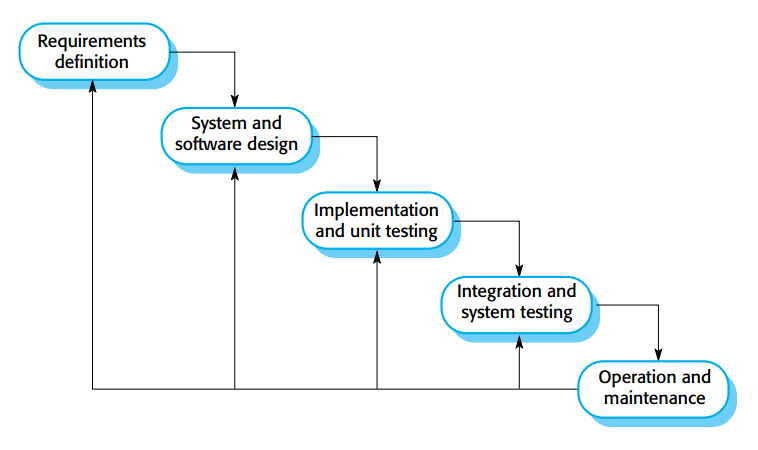
\includegraphics[width=.7\linewidth]{img/waterfall}
  \caption{Model \emph{waterfall} \parencite{sommerville2016software}}\label{fig:waterfall}
\end{figure}

\subsection{Arsitektur \emph{Model View Controller}}

\emph{Model-View-Controller (MVC)} merupakan sebuah model
infrastruktur yang memisahkan antara \emph{user interface} dari
fungsionalitas inti sistem. \emph{Model} memuat segala
\emph{content} dan fungsionalitas yang spesifik pada sistem yang
dibangun, \emph{processing logic} dan akses ke sumber informasi atau
data eksternal. \emph{View} memuat segala fungsi spesifik
\emph{interface}, dan segala proses fungsionalitas yang dibutuhkan
\emph{end-user}. \emph{Controller} mengatur akses ke
\emph{model} dan \emph{view} serta mengatur aliran data antara
keduanya \parencite{pressman2010software}. Penggunaan arsitektur \emph{MVC} akan
menghasilkan tiga \emph{class} utama, yaitu \emph{class view, model},
dan \emph{class controller}. \emph{Class model} akan memuat seluruh
fungsionalitas inti yang spesifik pada sistem. Hal ini memberikan
banyak keuntungan tatkala sistem akan dikembangkan lebih lanjut,
karena pada pengembangan selanjutnya pengembang cukup fokus pada bagian
\emph{controller} dan \emph{view}.

\subsection{Pendekatan Berorientasi Objek}

% sejarah, apa itu pendekatan berorientasi objek ?
Langkah awal yang signifikan terhadap desain berorientasi objek
terlahir dalam komunitas pengguna bahasa pemrograman \emph{Ada}. Hal
ini bermula ketika Grady Booch merasionalkan metode yang diciptakan
Russell J. Abbott pada tahun 1983. Grady Booch kemudian menyebut
karyanya sebagai \emph{object-oriented design}. Keduanya
merekomendasikan bahwa untuk memulai membangun desain berorientasi
objek, dimulai dari deskripsi informal dari sistem yang
akan dibangun. Dari deskripsi informal tersebut pengembang
sistem dapat mengidentifikasi \emph{class} dan objek dari kata benda dan
operasi dari kata kerja yang ditemukan. Beberapa waktu setelahnya
Grady Booch mengemukakan konsep baru yang tidak lagi berbasis pada
deskripsi naratif melainkan menggabungkan \emph{object-oriented
  design} dengan metodologi yang sudah ada, kemudian menyebutnya
sebagai \emph{object-oriented development}
\parencite{capretz2003history}.

Pada tahun 1990-an Grady Booch bersama dengan dua orang rekannya, yaitu
James Rumbaugh dan Ivar Jacobson mulai mengerjakan suatu metode yang
diharapkan bersifat universal. Metode tersebut dibangun berdasarkan
kombinasi dari fitur-fitur terbaik pada metode-metode
\emph{object-oriented analisis} dan \emph{design method} yang
ada. Metode ini juga mengadopsi fitur-fitur yang diajukan oleh ahli
lain dalam rekayasa perangkat lunak. Karya ketiga orang tersebut yang
dikenal sekarang dengan \emph{Unified Modeling
  Language} (\emph{UML}). \emph{UML} berisi notas-notasi yang dapat digunakan
untuk pemodelan dan pengembangan sistem berorientasi objek. Tujuh
tahun setelahnya, yaitu pada tahun 1997 \emph{UML} menjadi standar \emph{de
  facto} untuk membangun perangkat lunak berorientasi objek
\parencite{pressman2010software}.

Membangun perangkat lunak dengan pendekatan berorientasi objek
memiliki aktivitas \emph{object oriented analysis (OOA)} yang di
dalamnya terdapat proses ekstraksi \emph{class} atau \emph{object} dari
pernyataan kebutuhan. Selanjutnya terdapat aktivitas
\emph{object oriented design (OOD)} yang di dalamnya terdapat proses
\emph{refine} dan \emph{extend} \emph{class} yang didapatkan dari
\emph{OOA}. Dalam pengembangan ini umumnya terdapat \emph{boundary
  class} dan \emph{controller class}. \emph{Boundary class} bertindak
sebagai pembatas atau \emph{interface} antara pengguna dan
sistem. \emph{Boundary class} bertanggung jawab mengatur cara sebuah
entitas \emph{object} direpresentasikan kepada
pengguna. \emph{Controller class} mengatur pembuatan atau pembaharuan
pada entitas \emph{object}, penghubung antar \emph{boundary} dan data
yang didapatkan, dan komunikasi antar \emph{object} \parencite{pressman2010software}.


\subsection{Pemodelan Berorientasi Objek}

Notasi yang digunakan untuk pemodelan berorientasi objek adalah
\emph{Unified Modeling Language} (\emph{UML}). \emph{UML} merupakan
standar \emph{de facto} dalam pemodelan berorientasi objek. Terdapat
beberapa diagram inti dalam \emph{UML}, diantaranya adalah \emph{use
  case diagrams, sequence diagrams} dan \emph{class
  diagrams}. \emph{Use case diagrams} menunjukkan interaksi antar
pengguna dan sistem secara visual. \emph{Sequence diagrams}
menunjukkan interaksi antar komponen atau objek di dalam
sistem. \emph{Class diagrams} menunjukkan struktur sistem dan relasi antar
komponen pada sistem  \parencite{sommerville2016software}.

\subsubsection{\emph{Use Case Diagram}}

\emph{Use case diagram} merupakan sebuah diagram statis yang
menggambarkan interaksi antara pengguna dan sistem secara visual. \emph{Use case
  diagram} membantu menentukan fungsionalitas sebuah sistem dari
sudut pandang pengguna~\parencite{pressman2010software}. \emph{Use
  case diagram} tidak menggambarkan tahapan. \emph{Use case}
digambarkan dengan bentuk oval dan aktor digambarkan dengan gambar
orang (\emph{stick figure}). Notasi \emph{use case diagram}
dan deskripsinya dipaparkan pada Tabel~\ref{tab:notasi-use-case},
dan contoh \emph{use case diagram} terdapat dalam
Gambar~\ref{fig:contoh-use-case}.

\begin{longtable}{|>{\centering}m{5cm}|m{7cm}|}
  \caption{Notasi \emph{use case diagram} \parencite{rumbaugh2004unified}}\label{tab:notasi-use-case}
  \\\hline
  \textbf{Notasi} & \textbf{Deskirpsi} \\\hline
  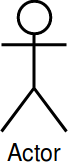
\includegraphics[width=.1\linewidth]{img/uml-notation/actor}
                         & Notasi aktor menggambarkan pengguna atau
                           sistem luar yang berinteraksi dengan
                           sistem. \\\hline
                           %
  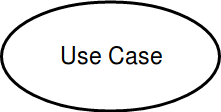
\includegraphics[width=.4\linewidth]{img/uml-notation/usecase}
                         & Notasi \emph{use case} merepresentasikan
                           fungsionalitas yang dapat dijalankan oleh
                           aktor. \\\hline
                           %
  
\includegraphics[width=.6\linewidth]{img/uml-notation/path}
                         & Notasi asosiasi merupakan jalur komunikasi
                           antara aktor dan \emph{use case}. \\\hline
                           %
  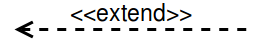
\includegraphics[width=.6\linewidth]{img/uml-notation/extends}
                         & Notasi \emph{extends} merupakan sisipan
                           fungsionalitas tambahan terhadap \emph{base
                           use case} yang tidak mengetahui sisipan
                           tersebut. \\\hline
                           %
  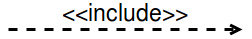
\includegraphics[width=.6\linewidth]{img/uml-notation/include}
                         & Notasi \emph{include} merupakan sisipan
                           fungsionalitas tambahan terhadap
                           \emph{basecase} yang secara eksplisit
                           menjelaskan sisipan tersebut. \\\hline
                           %
  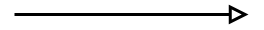
\includegraphics[width=.6\linewidth]{img/uml-notation/general}
                         & Notasi \emph{use case generalization}
                           merupakan relasi antara \emph{general use
                           case} dan \emph{specific use case} yang
                           mewarisi dan menambahkan fitur padanya. \\\hline
\end{longtable}

\begin{figure}[tph]
  \centering
  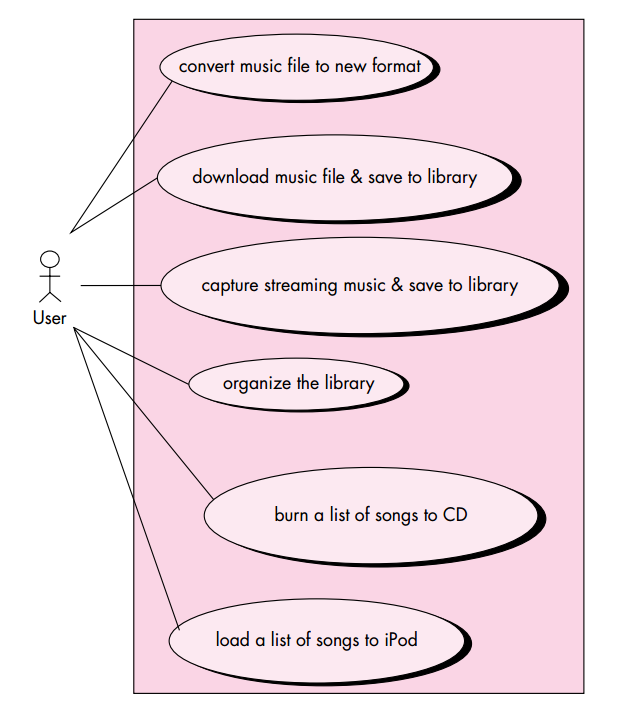
\includegraphics[width=.5\linewidth]{img/contoh-use-case}
  \caption{Contoh \emph{use case diagram} \parencite{pressman2010software}}\label{fig:contoh-use-case}
\end{figure}


\subsubsection{\emph{Sequence Diagram}}

\emph{Sequence diagram} merupakan sebuah diagram dinamis yang
menggambarkan interaksi antar objek di dalam sistem pada saat sistem
mengeksekusi sebuah tugas. Terjadi pertukaran \emph{messages} antar
objek pada sistem untuk menyelesaikan sebuah tugas
\parencite{pressman2010software}. Notasi \emph{sequence diagram} dan
deskripsinya terdapat pada Tabel~\ref{tab:notasi-sequence-diagram},
dan contoh \emph{sequence diagram} terdapat dalam
Gambar~\ref{fig:contoh-sequence-diagram}.

\begin{longtable}{|>{\centering}m{5cm}|m{7cm}|}
  \caption{Notasi \emph{sequence diagram}}\label{tab:notasi-sequence-diagram}\\
  \hline \textbf{Notasi} & \textbf{Deskirpsi} \\\hline
  
\includegraphics[width=.007\linewidth]{img/uml-notation/lifeline}
                         & Notasi \emph{lifeline} menggambarkan waktu
                           aktif (\emph{life}) suatu objek.\\\hline
                           %
  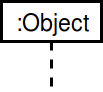
\includegraphics[width=.2\linewidth]{img/uml-notation/objek}
                         & Notasi \emph{object} merepresentasikan objek
                           yang berinteraksi dengan objek lainnya. \\\hline
                           %
  
\includegraphics[width=.04\linewidth]{img/uml-notation/activation-bar}
                         &Notasi \emph{activation bar}
                           merepresentasikan lama suatu objek aktif
                           berinteraksi.\\\hline
                           %
  
\includegraphics[width=.6\linewidth]{img/uml-notation/invoke}
                         & Notasi \emph{method invocation}
                           merepresentasikan suatu \emph{method} dari
                           sebuah objek yang panggil oleh objek
                           lainnya.\\\hline
                           %
  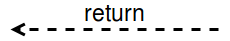
\includegraphics[width=.6\linewidth]{img/uml-notation/return}
                         & Notasi \emph{return} merepresentasikan data
                           yang dikembalikan oleh method \emph{calle}
                           kepada method \emph{caller}.\\\hline
                           %
  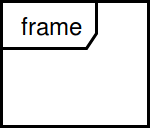
\includegraphics[width=.4\linewidth]{img/uml-notation/frame}
                         & Notasi \emph{frame} menggambarkan lingkup
                           suatu interaksi dengan interaksi lainnya
                           atau lingkup suatu interaksi dan dunia luar. \\\hline
                         %
  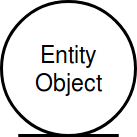
\includegraphics[width=.3\linewidth]{img/uml-notation/entity}
                         & Notasi \emph{entity object} merepresentasikan
                           objek yang bertanggung jawab untuk mengatur
                           data dalam sebuah sistem. \\\hline
                         %
  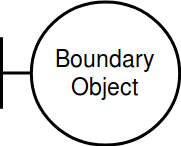
\includegraphics[width=.3\linewidth]{img/uml-notation/boundary}
                         & Notasi \emph{boundary object} merepresentasikan
                           objek yang bertanggung jawab untuk mengatur
                           alur sebuah objek direpresentasikan kepada aktor. \\\hline
                         %
  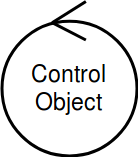
\includegraphics[width=.3\linewidth]{img/uml-notation/control}
                         & Notasi \emph{controller object}
                           merepresentasikan suatu objek yang mengatur
                           pembuatan atau pembaharuan entitas
                           \emph{object}, penghubung antar
                           \emph{boundary} dan \emph{entity} dan
                           komunikasi antar \emph{object}. \\\hline

\end{longtable}

\begin{figure}[tph]
  \centering
  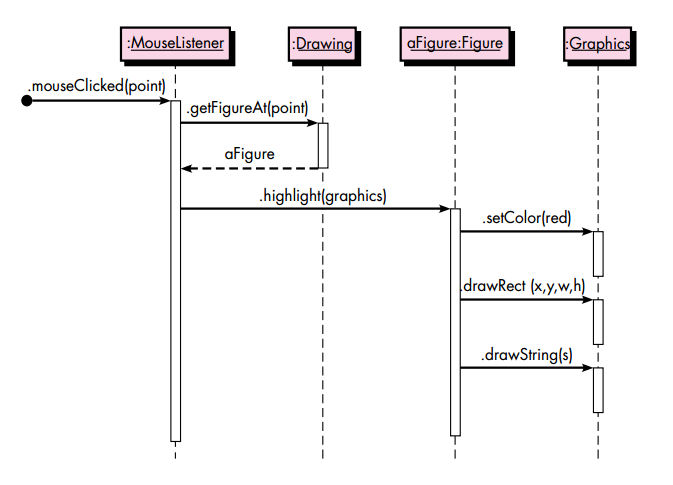
\includegraphics[width=.7\linewidth]{img/contoh-sequence}
  \caption{Contoh \emph{sequence diagram} \parencite{pressman2010software}}
   \label{fig:contoh-sequence-diagram}
\end{figure}


\subsubsection{\emph{Class Diagram}}

\emph{Class diagram} merupakan sebuah diagram statis atau \emph{structural view}
yang memodelkan \emph{class}, \emph{class attribute}, \emph{class operation},
hubungan, dan asosiasi antar \emph{class}. Elemen utama dari \emph{class
  diagram} adalah kotak yang terbagi menjadi beberapa bagian. Bagian atas
merepresentasikan nama \emph{class}, bagian tengah merepresentasikan
\emph{attribute}, dan bagian bawah merepresentasikan
\emph{operation}. \emph{Attribute} merupakan apa yang sebuah \emph{class} atau
objek ketahui, \emph{operation} merupakan apa yang sebuah \emph{class} atau
objek dapat lakukan~\parencite{pressman2010software}. Notasi dan deskripsi dari
notasi tersebut dipaparkan pada Tabel~\ref{tab:notasi-class-diargam}, dan Contoh
dari \emph{class diagram} terdapat dalam Gambar~\ref{fig:contoh-class-diagram}.

\begin{longtable}{|>{\centering}m{5cm}|m{7cm}|}
  \caption{Notasi \emph{class diagram}}\label{tab:notasi-class-diargam}\\
  \hline \textbf{Notasi} & \textbf{Deskirpsi} \\\hline
  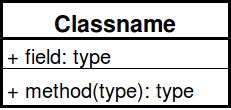
\includegraphics[width=.44\linewidth]{img/uml-notation/class}
                         & Notasi \emph{class} merepresentasikan suatu
                           \emph{class} yang berisikan
                           \emph{attribute} dan \emph{method}.\\\hline
                           %
  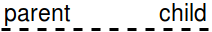
\includegraphics[width=.6\linewidth]{img/uml-notation/association-class}
                         & Notasi \emph{association} menggambarkan
                           hubungkan antar suatu \emph{class} dengan
                           \emph{class} lainnya. \\\hline
                           %
  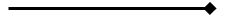
\includegraphics[width=.6\linewidth]{img/uml-notation/composition-class}
                         & Notasi \emph{composition} menggambarkan
                           hubungan kuat antar suatu \emph{class} dengan
                           \emph{class} lain, di mana keduanya
                           saling membutuhkan secara kuat dan saling
                           membutuhkan. \\\hline
                           %
  
\includegraphics[width=.6\linewidth]{img/uml-notation/agregation-class}
                         & Notasi \emph{agregation} menggambarkan
                           hubungan lemah antar suatu \emph{class}
                           dengan \emph{class} yang lain, di mana
                           keduanya tidak saling membutuhkan atau keduanya bisa
                           berdiri sendiri. \\\hline
                           %
  
\includegraphics[width=.6\linewidth]{img/uml-notation/generalization-class}
                         & Notasi \emph{generalization}
                           merupakan relasi antara \emph{parent class}
                           dan \emph{child class}, di mana \emph{child class}
                           mewarisi dan menambahkan fitur dari
                           \emph{parent class}. \\\hline
                           %
\end{longtable}

\begin{figure}[tph]
  \centering
  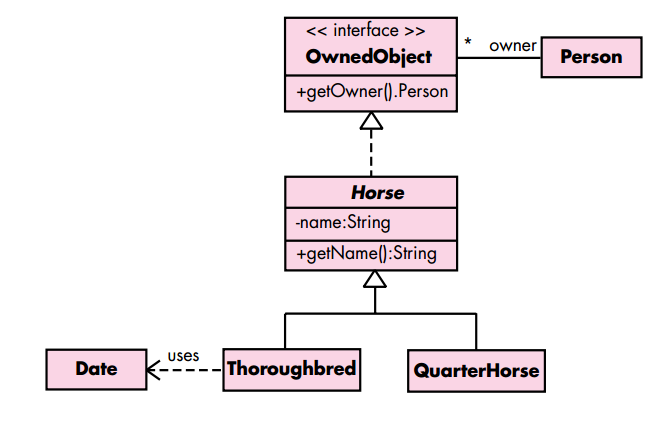
\includegraphics[width=.6\linewidth]{img/contoh-class}
  \caption{Contoh \emph{class diagram} \parencite{pressman2010software}}
  \label{fig:contoh-class-diagram}
\end{figure}


\subsection{Pengujian Perangkat Lunak}

% kapan pengujian itu ada
% apa kekurangan dan kelebihan
% metode yang digunakan apa aja

Penggunaan perangkat lunak yang masif tanpa adanya standardisasi
membuat \emph{IEEE} mempublikasikan sebuah \emph{issue} pada bulan november
hingga desember di tahun 1999. \emph{IEEE} dan \emph{ACM} kemudian
membentuk tim gabungan untuk mendefinisikan standardisasi pada proses
pengembangan perangkat lunak. Standardisasi tersebut memuat tentang
\emph{scientific principles, engineering processes, standards,
  methods, tools, measurement} dan \emph{best practices}, proses pengujian
atau \emph{testing} termasuk di dalamnya \parencite{burnstein2006practical}.

Pengujian bertujuan untuk menemukan cacat dan menguji kualitas suatu
perangkat lunak. Dalam proses pengujian terdapat beberapa tahapan, metode, dan
teknik. Setiap komponen pada bagian-bagian tersebut memiliki
kelemahan dan kekurangan tertentu. Proses testing juga akan
menghasilkan artefak-artefak seperti \emph{test-scenario, test-case,
  test-data} dan \emph{test scripts} \parencite{burnstein2006practical}.

\subsubsection{Tahapan Pengujian}

Terdapat beberapa tahapan dalam pengujian. Tahapan-tahapan tersebut
diantaranya \emph{unit testing, integration testing}, dan \emph{validation
  testing} \parencite{presman2010software}. Tahapan awal dalam pengujian adalah
tahapan pengujian \emph{unit}. Terdapat beberapa
pendapat berbeda mengenai ``\emph{unit}'' dalam \emph{unit
  testing}. \textcite{martin2014unittest} berpendapat bahwa definisi
\emph{unit} dapat berarti \emph{single method, single class} maupun
kumpulan dari beberapa \emph{class}. \textcite{osherove2015art} tidak
mengikat definisi \emph{unit} pada \emph{class} maupun
\emph{method}, melainkan mengikatnya dengan definsi atribut seperti
\emph{performance, reliability} dan \emph{consistency}. \emph{Google}
tidak menggunakan istilah \emph{unit, integration} ataupun
\emph{system} untuk merujuk pada tingkatan tertentu, melainkan
menggunakan istilah \emph{small, medium, large}
\parencite{whittaker2012google}. Di sisi lain,
\textcite{presman2010software} berpendapat bahwa fokus pengujian
\emph{unit} pada perangkat lunak konvensional adalah sebuah modul dan
fokus pengujian \emph{unit} pada perangkat lunak berorientasi objek
adalah \emph{class} dengan \emph{testable unit} terkecil adalah
\emph{operation} atau \emph{method}. Tahapan selanjutnya adalah \emph{Integration
  testing}. \emph{Integrartion testing} merupakan pengujian yang
dilakukan pada kumpulan \emph{unit} yang telah diuji. Hal ini
dilakukan untuk memastikan suatu \emph{unit} akan berjalan dengan baik
jika dijalankan bersamaan dengan \emph{unit} yang lain. Meskipun
setiap \emph{unit} telah diuji secara individu, terdapat beberapa
kemungkinan galat yang terjadi ketika \emph{unit-unit} tersebut diuji
secara bersamaan. Beberapa kemungkinan galat yang akan terjadi di
antaranya adalah hilangnya data ketika melintasi \emph{interface}, dan
komponen yang tidak berjalan semestinya ketika digabungkan. Pada
proses pengujian \emph{unit} maupun \emph{integrartion}, komponen
tidak berupa \emph{stand-alone program}. Maka dibutuhkan pembuatan
\emph{stub} ataupun \emph{driver} selama proses pengujian.
\emph{Driver} hanyalah \emph{main program} tiruan yang menjalankan
kasus uji, sedangkan \emph{stub} merupakan sebuah \emph{dummy
  subprogram} yang bekerja menggantikan komponen-komponen pengujian
yang asli.

Pada sistem dengan arsitektur berorientasi objek pengujian integrasi
dengan pendekatan \emph{incremental top-down integration} maupun
\emph{incremental bottom-up integration} tidak dapat digunakan,
karena sistem berorientasi objek tidak memiliki kontrol hierarki
yang jelas. Maka dibutuhkan pendekatan yang berbeda, yaitu dengan
pendekatan integrasi \emph{thread-based testing} dan \emph{use-based
  testing}. \emph{Thread-based testing} bekerja dengan
mengintegrasikan sekumpulan \emph{class} yang dibutuhkan untuk \emph{input}
tertentu. Setiap \emph{thread} diuji dan diintegrasikan secara
individu. \emph{Use-based testing} berkeja dengan menguji
\emph{class} independen yang memiliki ketergantungan paling kecil
dengan \emph{class} lainnya. Setelah \emph{class}-\emph{class}
tersebut diuji, lapisan \emph{class} selanjutnya (\emph{dependent
  classess}) yang menggunakan \emph{independent class} diuji hingga
seluruh sistem selesai diuji \parencite{presman2010software}. Tahapan terakhir adalah pengujian
validasi atau \emph{validation testing}. Pengujian validasi fokus
terhadap \emph{user-visible action} dan \emph{user-recognizable
  output} dari sistem, atau dengan kata lain pengujian validasi
menguji apakah sistem yang dibangun sudah sesuai dengan seluruh
skenario kebutuhan yang didefinisikan~\parencite{pressman2010software}. Tahapan pengujian
terlihat dalam Gambar~\ref{fig:testing-level}.

\begin{figure}[H]
  \centering
  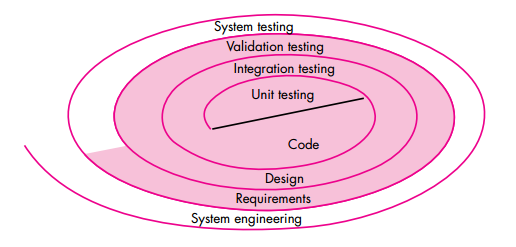
\includegraphics[width=.7\linewidth]{img/tahapan-pengujian}
  \caption{Tahapan pengujian \parencite{presman2010software}}\label{fig:testing-level}
\end{figure}

\subsubsection{Metode Pengujian}

Metode pengujian atau \emph{point of view} dalam pengujian merupakan
sudut pandang seorang \emph{tester} tatkala mendesain sebuah
\emph{test case}. Terdapat di antaranya \emph{white-box testing} dan
\emph{black-box testing}. Kedua metode tersebut memiliki kekurangan
masing-masing. Metode \emph{white-box testing} tidak dapat menemukan
kebutuhan yang belum diimplementasikan
\parencite{dijkstra1970notes}. Hal ini dapat diselesaikan dengan
penggunaan metode \emph{black-box testing}. Begitu juga dengan
kekurangan metode \emph{black-box testing} yang dapat menghasilkan
\emph{test-case} yang tidak tepat dan tidak dapat menemukan bagian
yang belum diuji \parencite{savenkov2008become}. Kelemahan pada metode
\emph{black-box testing} ini dapat diselesaikan dengan menggunakan
metode \emph{white-box testing}. Oleh karena itu, penggunaan kedua metode
dalam pengujian sistem menyelesaikan semua masalah pada masing-masing kekurangan
yang dimiliki kedua metode.

\emph{White-box testing} merupakan suatu metode pengujian di mana
proses pengujiannya dilakukan dengan melihat internal perangkat lunak.
Maka pada tahapan ini seorang penguji wajib memiliki kemampuan
pemrograman. Pengujian ini dilakukan untuk menguji apakah \emph{logic}
dan \emph{data} pada perangkat lunak berfungsi sebagaimana mestinya
\parencite{myers2011art}. Di sisi lain \emph{black-box testing} hanya
menguji bagian luar suatu perangkat lunak. Pada tahapan ini
fungsionalitas suatu perangkat lunak diuji tanpa harus mengetahui
internalnya. Oleh karena itu, tidak dibutuhkan kemampuan pemrograman
saat membuat \emph{test case} pada pengujian \emph{black-box}. Penguji
hanya mengetahui bagaimana seharusnya perangkat lunak berjalan
(\emph{what}), bukan bagaimana perangkat lunak itu melakukan sesuatu
(\emph{how}). Pada tahapan ini penguji hanya mempertimbangkan masukan
(\emph{input}) dan keluaran (\emph{output}) perangkat lunak selama
mendesain \emph{test-case} \parencite{myers2011art}.


\subsubsection{Teknik Pengujian}

Terdapat beberapa teknik dalam pengujian. Pengujian semua \emph{path}
atau \emph{rigorous testing} pada proses \emph{white-box testing}
tidak mungkin dilakukan sehingga digunakan teknik \emph{basis path
testing} untuk menentukan \emph{path} yang akan diuji
\parencite{gregory2007path}. \emph{Rigorous testing} atau
\emph{exhaustive testing} (\emph{C$\infty$}) atau menguji semua
kemungkinan juga tidak mungkin dilakukan pada saat pengujian
\emph{black-box} sehingga penggunaan teknik \emph{equivalence
partitioning} untuk menentukan masukan yang \emph{valid} dan
\emph{invalid} diperlukan. Teknik \emph{boundary value analysis}
menjadi pelengkap teknik \emph{equivalence
partitioning}. \emph{Boundary value analysis} digunakan untuk
mendapatkan nilai masukan yang berada pada \emph{boundary} atau
\emph{corner}, karena nilai-nilai pada bagian tersebut memiliki
kemungkinan galat yang besar \parencite{presman2010software}. Maka tiga teknik
utama dalam pengujian perangkat lunak adalah:

\begin{enumerate}
\item \emph{Basis path testing}
\item \emph{Equivalence partitioning}
\item \emph{Boundary value analysis }
\end{enumerate}

\emph{Basis path testing} merupakan suatu teknik pengujian pada metode
\emph{white-box} yang diajukan oleh McCabe pada tahun 1996. Teknik ini
menggunakan penelitian McCabe yang sebelumnya yaitu \emph{cyclomatic
complexity} yang ia temukan pada tahun 1976. Meski saat ini \emph{cyclomatic
complexity} banyak dikaitkan secara erat dengan rumus untuk menentukan
jumlah \emph{independent path}. \emph{Cyclomatic complexity} yang awalnya
ditemukan pada tahun 1976 diajukan untuk mengukur tingkat kompleksitas
suatu modul dalam sebuah program. Modul yang melebihi nilai
\emph{cyclomatic complexity} sepuluh direkomendasikan untuk dipisah atau
dilakukan \emph{refactoring}. Tujuan kedua dari rumus tersebut adalah
untuk melihat tingkat terstrukturnya (\emph{structuredness}) suatu
modul. Hal yang membuat \emph{cyclomatic complexity} dikaitkan secara
erat dengan proses \emph{basis path testing} karena kemudian McCabe
sadar bahwa \emph{cyclomatic complexity} dapat menemukan
\emph{independent path} pada suatu modul. \emph{Independent path} adalah
suatu jalur dalam sebuah program yang memperkenalkan setidaknya suatu rangkaian
pemrosesan baru atau kondisi baru. Hal tersebut yang
mengantarnya pada pengajuan \emph{basis path testing} pada tahun 1996.
\emph{Basis path testing} memiliki keunggulan karena V(G) atau
\emph{vector space} memiliki nilai yang menjadi batas atas \emph{upper
bound} untuk membuat \emph{test-case} pada suatu program. Hal ini
menguntungkan penguji karena dapat menentukan ukuran batas selesainya
suatu pengujian. Selain itu, \emph{basis path testing} memiliki nilai
yang lebih baik dari pada \emph{branch coverage}, yaitu \emph{branch
  coverage ≤ cyclomatic complexity ≤ all of paths} \parencite{gregory2007path}.
Langkah-langkah pengujian \emph{basis path} adalah sebagai berikut \parencite{presman2010software}:

\begin{enumerate}[
leftmargin=0pt, itemindent=20pt,
labelwidth=15pt, labelsep=5pt, listparindent=0.7cm,
align=left]
\item Membuat \emph{flow graph} dari desain atau \emph{code}.

  \emph{Flow graph} memiliki beberapa notasi seperti \emph{sequence,
    if, while, until} dan \emph{case}. Gambar notasi-notasi tersebut
  terlihat pada Gambar~\ref{fig:notasi-flow-graph}. Terlihat \emph{flow graph}
  pada Gambar~\ref{cfg:hallo} yang dihasilkan dari
  \emph{pseudocode}~\ref{ps:hallo}.

\item Menentukan \emph{cyclomatic complexity} dari \emph{flow graph}
  yang dihasilkan.

  \emph{Cyclomatic complexity} adalah suatu metrik perangkat lunak
  yang memberikan ukuran kuantitatif kompleksitas logis dari suatu
  program. \emph{Cyclomatic complexity} dapat ditentukan dengan menggunakan
  rumus~\ref{eq:perhitungan-cc}:

  \begin{equation}
    \begin{array}{l}
      V(G) = jumlah \thinspace region \\
      V(G) = E – N + 2 \\
      V(G) = P + 1, \thinspace di mana \thinspace P – predicate \thinspace node
    \end{array}\label{eq:perhitungan-cc}
  \end{equation}

  Maka Perhitungan \emph{cyclomatic complexity} yang dilakukan pada
  \emph{flow graph}~\ref{cfg:hallo} menghasilkan
  nilai sebagai berikut:

  \begin{equation}
    \begin{array}{l}
      V(G) = 2 \thinspace regions \\
      V(G) = 4 \thinspace edges \thinspace – \thinspace 4 \thinspace
      nodes \thinspace + \thinspace 2 \thinspace = \thinspace 2 \\
      V(G) = 1 \thinspace predicate \thinspace node \thinspace +
      \thinspace 1 \thinspace = \thinspace 2
    \end{array}\label{eq:hasil-perhitungan-cc}
  \end{equation}

 Jadi, \emph{flow graph} pada Gambar~\ref{cfg:hallo} memiliki nilai
 \emph{cyclomatic complexity} = 2.

\item Menentukan \emph{independent path}.

  \emph{Independent path} adalah suatu jalur dalam sebuah program yang
  memperkenalkan setidaknya suatu rangkaian pemrosesan baru atau
  kondisi baru. Nilai dari V(G) memberikan batas atas dari banyaknya
  \emph{independent path} dari sebuah program. Dari contoh
  \emph{pseudocode} \emph{procedure hallo} kita mendapatkan 2 jalur
  \emph{independent} sebagai berikut: \par\null\par

  Jalur 1: 1 - 2 - 4 \par
  Jalur 2: 1 - 3 - 4

\item Membuat \emph{test case} yang akan menjalankan setiap jalur pada
  \emph{basis path}.

  Terdapat dua \emph{test case} yang akan dihasilkan. Pertama
  \emph{test case} yang harus melewati jalur 1 sehingga pada \emph{test
    case} pertama nilai \emph{variable nama} harus bernilai
  \emph{true}. Pada \emph{test case} kedua nilai \emph{variable nama}
  harus bernilai \emph{false} agar jalur 2 dijalankan. \emph{Test case}
  yang dihasilkan tampak seperti pada Tabel~\ref{tc:hallo}.

\end{enumerate}

\begin{figure}[H]
  \centering
  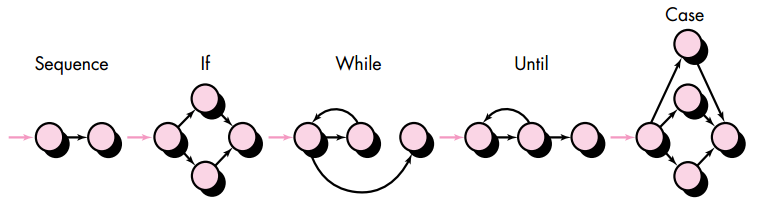
\includegraphics[width=.8\linewidth]{img/notasi-flow-graph}
  \caption{Notasi \emph{flow graph} \parencite{presman2010software}}\label{fig:notasi-flow-graph}
\end{figure}


\begin{center}
\begin{minipage}{0.8\textwidth}
\begin{code}
\begin{ignasicblock}[title=hallo,minted language=text]
procedure hallo(nama)
   IF nama == "Budi"          (1)
      RETURN "Hai" + nama     (2)
   ELSE
      RETURN "Nama kosong"    (3)
   ENDIF                      (4)
end
\end{ignasicblock}
\captionof{listing}{Contoh \emph{pseudocode}}\label{ps:hallo}
\end{code}
\end{minipage}
\end{center}

\begin{figure}[H]
  \centering
  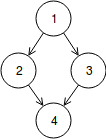
\includegraphics[width=.14\linewidth]{img/contoh-flow-graph}
  \caption{Representasi \emph{control flow graph} dari \emph{pseudocode}~\ref{ps:hallo}}\label{cfg:hallo}
\end{figure}

\begin{longtable}{|P{.06\textwidth}|P{.30\textwidth}|P{.30\textwidth}|P{.10\textwidth}|P{.08\textwidth}|}
  \caption{\emph{Test case} dari contoh \emph{pseudocode}~\ref{ps:hallo}} \label{tc:hallo}\\
  \hline
  \textbf{Jalur} & \textbf{Prosedur Uji} & \textbf{\emph{Expected Result}} \\\hline
  %
  1 & Memberikan nilai \emph{``Budi''} pada variable \emph{nama} &
                                                                   Program menampilkan ``Hai Budi'' \\\hline
                                                                   %
  2 & Tidak memberikan nilai apapun pada variable \emph{nama} &
                                                                   Program menampilkan ``Nama kosong'' \\\hline
  %

\end{longtable}


\emph{Equivalence partitioning} merupakan suatu teknik dalam metode
pengujian \emph{black-box} di mana prosesnya adalah membagi masukan
kepada kelas-kelas data. Dari kelas-kelas tersebut \emph{test case}
nantinya didapatkan. \emph{Equivalence class} merepresentasikan
keadaan valid atau tidak validnya suatu masukan. Beberapa kondisi
masukan di antaranya \emph{numeric value, range of values, set of
related values,} atau \emph{boolean condition}. \emph{Equivalence
partitioning} dapat di definisikan sesuai dengan panduan berikut
\parencite{presman2010software}:

\begin{enumerate}[
leftmargin=0pt, itemindent=20pt,
labelwidth=15pt, labelsep=5pt, listparindent=0.7cm,
align=left]

\item Jika kondisi masukan adalah \emph{range}. Maka satu valid dan
  dua invalid \emph{equivalence class} di definisikan.
\item Jika kondisi masukan adalah \emph{specific value}. Maka satu valid dan
  dua invalid \emph{equivalence class} di definisikan.
\item Jika kondisi masukan adalah \emph{member of a set}. Maka satu valid dan
  satu invalid \emph{equivalence class} di definisikan.
\item Jika kondisi masukan adalah \emph{boolean}. Maka satu valid dan
  satu invalid \emph{equivalence class} di definisikan.

\end{enumerate}

Jika data masukan bertipe \emph{range} dan masukan yang valid adalah
\emph{range} bernilai 4 hingga 10. Maka masukan yang tidak valid
adalah semua angka yang kurang dari 4 dan semua angka yang lebih dari
10 seperti terlihat pada Gambar~\ref{fig:contoh-ep-marked}. Data
yang digunakan untuk \emph{test case} pada tipe masukan \emph{range}
berjumlah 3. Satu bernilai valid dan dua bernilai invalid. Oleh karena itu,
data masukan \emph{valid} yang kita gunakan adalah 11 dan 7. Sedangkan
data \emph{invalid} yang digunakan adalah 3.

\begin{figure}[H]
  \centering
  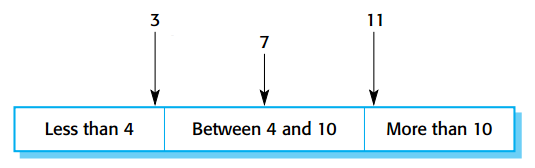
\includegraphics[width=.6\linewidth]{img/contoh-ep-marked}
  \caption{Contoh \emph{equivalence partitioning} \parencite{sommerville2016software}}\label{fig:contoh-ep-marked}
\end{figure}

\emph{Boundary value analysis} merupakan suatu teknik yang melengkapi
\emph{equivalence partitioning}. \emph{Boundary value analysis}
dikembangkan untuk menganalisis nilai yang berada pada \emph{boundary}
\emph{input}, karena nilai pada \emph{boundary} atau \emph{corner} memiliki
peluang galat yang lebih tinggi. \emph{Boundary value analysis} tidak
berdiri sendiri, melainkan merupakan teknik yang melengkapi
\emph{equivalence partitioning}. Maka \emph{boundary value analysis}
mengambil nilai yang bersifat ``pojok'' dari nilai hasil
\emph{equivalence partitioning}. Panduan pemilihan nilai
\emph{boundary value analysis} di antaranya sebagai berikut
\parencite{presman2010software}:

\begin{enumerate}[
leftmargin=0pt, itemindent=20pt,
labelwidth=15pt, labelsep=5pt, listparindent=0.7cm,
align=left]

\item Jika masukan merupakan sebuah \emph{range} dari a hingga
  b. Maka nilai yang digunakan untuk \emph{test case} adalah satu
  nilai di atas a dan satu nilai di bawah b.
\item Jika masukan merupakan sebuah \emph{number of values}. Maka
  nilai yang digunakan untuk \emph{test case} adalah nilai maksimum
  dan minimum serta satu nilai di atas maksimum dan satu nilai di
  bawah minimum.
\end{enumerate}

Jika data masukan bertipe \emph{range} dari 4 hingga 10. Maka nilai
yang didapatkan untuk pengujian adalah nilai maksimum dan minimum
serta satu nilai di atas maksimum dan satu nilai di atas minimum. Jadi
nilai yang didapatkan adalah 4, 10, 3, dan 11 seperti terlihat pada
Gambar~\ref{fig:contoh-bva-marked}.

\begin{figure}[H]
  \centering
  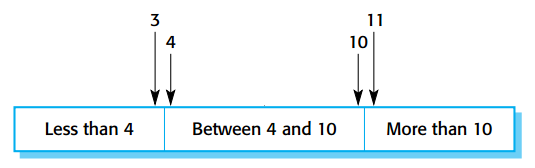
\includegraphics[width=.6\linewidth]{img/contoh-bva-marked}
  \caption{Contoh \emph{boundary value analysis}
    \parencite{sommerville2016software}}\label{fig:contoh-bva-marked}
\end{figure}

\subsubsection{\emph{Automated Testing}}

Menjalankan semua \emph{test case} secara manual sangat menyita
waktu. Bahkan mereka dapat menyita 50\% dari pada waktu pengembangan
\parencite{brooks1995mythical}. \emph{Automated testing} dapat
digunakan untuk mempercepat proses pengujian. \emph{Automated testing}
adalah proses menjalakan \emph{test case} secara otomatis.
\emph{Automated testing} berjalan dengan adanya \emph{trigger}, baik
dalam bentuk \emph{event} maupun \emph{time}. Prosesnya adalah dengan
menjalankan \emph{test case} dan membandingkannya dengan \emph{output}
yang sudah ditentukan. Hasil perbandingan tersebut akan dilaporkan
kepada penguji secara otomatis setelah \emph{automated testing}
selesai dijalankan \parencite{marcellintravis}. \emph{Automated
  testing} dibangun dengan menggunakan \emph{script} sesuai dengan
\emph{test case} yang didapatkan dari tahapan pengujian
\emph{white-box} maupun \emph{black-box}. Tampak pada Tabel
Kode~\ref{ts:hallo} merupakan \emph{script} yang dibangun untuk
melakukan pengujian secara otomatis. \emph{Script} tersebut didapatkan dari
\emph{test case} untuk pengujian \emph{pseudocode hallo} pada Tabel
Kode~\ref{tc:hallo}. \emph{Script} ini nantinya dijalankan dengan
kakas bantu \emph{Pytest} untuk melakukan pengecekan berhasil atau
gagalnya suatu pengujian secara otomatis. Sedangkan \emph{trigger} untuk
menjalankan \emph{Pytest} secara otomatis dilakukan dengan bantuan
kakas bantu \emph{Gitlab-CI}.

\begin{center}
\begin{minipage}{0.8\textwidth}
\begin{code}
\begin{ignasicblock}[title=test\_hallo,minted language=Python]
      def test_case_1():
          assert hallo("Budi") == "Hai Budi"

      def test_case_2():
          assert hallo("Ani") == "Nama Kosong"
\end{ignasicblock}
\captionof{listing}{Contoh \emph{script atomated testing}}\label{ts:hallo}
\end{code}
\end{minipage}
\end{center}

\subsubsection{Pengujian \emph{Compatibility}}

Pengujian \emph{compatibility} adalah pengujian yang dilakukan pada sistem yang
dibangun di atas beberapa media yang berbeda, seperti di atas \emph{display
  devices, operating systems} dan \emph{browser} yang
berbeda-beda. Masalah \emph{compatibility} yang kecil tidak memberikan
dampak signifikan pada sistem, tetapi masalah yang besar dapat
mengakibatkan dampak besar \parencite{pressman2010software}. Terdapat berbagai macam \emph{desktop
  environment} yang berbeda-beda pada sistem operasi \emph{GNU/Linux}. Setiap
\emph{desktop environment} memiliki format nama \emph{window} tersendiri. Sebuah
sistem harus dapat menangani perbedaan format nama \emph{window} agar dapat
\emph{compatible} antar \emph{desktop environment}. Pengujian \emph{compatibility}
terhadap perbedaan format nama \emph{window} antar \emph{desktop environment}
dilakukan dengan menjalankan sistem pada berbagai \emph{desktop environment} yang berbeda. Pengujian
berhasil jika sistem dapat menangani perbedaan format-format tersebut.
Beberapa format nama \emph{window} pada \emph{desktop environment} di antaranya:

\begin{itemize}
\item ``\_NET\_ACTIVE\_WINDOW(WINDOW): window id \# 0x3c00009''
\item ``\_NET\_ACTIVE\_WINDOW(WINDOW): window id \# 0x4a0000c, 0x0''
\end{itemize}

% teori teori apa saja yang dipakai.
%% activity logging, snapshotting, edit distance
\section{\emph{Snapshotting}}

% istilah snapshot sebenarnya datang dari analogi \emph{screenshot}
% dari dunia fotografi.
\emph{Snapshot} merupakan proses untuk merekam suatu keadaan media
penyimpanan dalam suatu waktu tertentu. \emph{Snapshot} yang
dihasilkan dapat dikembalikan kapan pun pengguna butuhkan. Umumnya
\emph{snapshot} dapat dihasilkan dari beberapa kakas bantu seperti
\emph{data protection software, data analisys}, dan \emph{replication
  aplication}. Implementasi untuk melakukan \emph{snapshot}
berbeda-beda, tergantung pada kebutuhan aplikasi\parencite{garimella}.
\emph{Version Control Software} (\emph{VCS})
merupakan salah satu kakas bantu yang dapat digunakan untuk membuat
\emph{snapshot}. \emph{VCS} lahir dimulai dengan adanya \emph{Source Code Control System (SCCS)}
pada tahun 1972 yang dibangun oleh Marc J. Rochkind, disusul
kemunculan \emph{Revision Control System (RCS)} pada tahun 1980,
\emph{Concurrent Versions System (CVS)} pada tahun 1985,
kemudian \emph{subversion} dan \emph{git} pada tahun-tahun berikutnya
\parencite{ruparelia2010history}

% https://git-scm.com/book/en/v2/Appendix-C%3A-Git-Commands-Basic-Snapshotting
\emph{Git} merupakan salah satu \emph{version control software} yang digunakan
secara umum. Hal ini disebabkan karena \emph{git} memiliki sifat
\emph{distributed} sehingga memiliki kelebihan yang tidak dimiliki
\emph{version control} terpusat, salah satunya adalah kemampuan untuk
melakukan seluruh operasi secara lokal \parencite{ruparelia2010history}.
\emph{Snapshot} pada \emph{git} disimpan di dalam \emph{repository} dan digunakan
untuk menyimpan suatu berkas dalam keadaan tertentu. Proses pembuatan \emph{snapshot} dapat
dilakukan dengan meminta \emph{git} untuk menambahkan semua
berkas yang ada menggunakan perintah ``\emph{add}''. Proses selanjutnya dilakukan dengan
menyimpan \emph{snapshot} secara permanen dengan menggunakan perintah
``\emph{commit}''. Proses ini akan menyimpan \emph{snapshot}
secara permanen pada \emph{database} \emph{git}.  Perintah lainnya yang dapat
kita gunakan adalah ``\emph{log}'' untuk melihat \emph{history} dari
\emph{snapshot}, dan ``\emph{diff}'' untuk melihat perbedaan antar
\emph{snapshot} \parencite{chacon2014pro}.

% how object stored Git benar-benar mengubah paradigma dunia e{version
Umumnya \emph{version control} beroperasi dengan menyimpan \emph{diff}
antar berkas pada suatu saat tertentu, cara ini biasa disebut dengan
\emph{delta-based version control}. Hal ini berbeda dengan \emph{git} yang menyimpan
keseluruhan \emph{snapshot} pada suatu waktu tertentu. Setiap
``\emph{commit}'' akan menyimpan seluruh keadaan berkas, kecuali
berkas yang tidak berubah. \emph{Git} melihat \emph{project} layaknya
\emph{stream of snapshots}. Semua \emph{snapshot} tersebut memiliki
integritas yang berupa 40 karakter \emph{hexadecimal} dihasilkan dari
kalkulasi berkas pada suatu \emph{snapshot} dengan algoritme
\emph{SHA-1}. Dengan \emph{hash} tersebut, \emph{git} dapat merujuk
suatu \emph{snapshot} tertentu \parencite{chacon2014pro}.

\begin{figure}[tph]
  \centering
  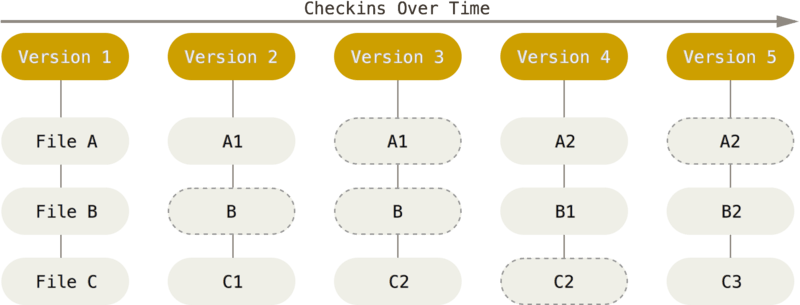
\includegraphics[width=.7\linewidth]{img/snapshots}
  \caption{Penyimpanan data sebagai \emph{snapshot} dari waktu ke
    waktu~\parencite{chacon2014pro}}\label{fig:snapshots}
\end{figure}


\section{\emph{User Activity Logging}}

% apa itu log ?
\emph{Log} merupakan sebuah berkas yang memuat rekaman semua aktivitas
yang terjadi pada perangkat lunak yang sedang berjalan. Pada
umumnya \emph{log} memiliki format berupa \emph{plain text} dan memuat
informasi berupa waktu, kategori dan deskripsi. \emph{Log} secara umum
digunakan pada \emph{web server, operating system} dan berbagai macam
perangkat lunak lain. Merekam aktivitas perangkat lunak maupun
pengguna dan menyimpannya ke dalam \emph{log} bertujuan untuk
melakukan \emph{debugging, monitoring, optimization, forensic
  analysis} dan beberapa tujuan lain. \emph{Log} memiliki beberapa
macam tipe, di antaranya \emph{event logs, message logs} dan
\emph{transaction log} \parencite{delarosa}.

% apa itu user activity logging ?
\emph{User activity logging} adalah sebuah proses menyimpan aktivitas pengguna ke dalam
sebuah \emph{log}. \emph{User activity} merupakan aktivitas pengguna dalam menggunakan
perangkat lunak. \emph{User activity} diantaranya adalah \emph{keystrokes}, gerakan
\emph{mouse}, suara, gerakan, gerakan mata, tempat yang dikunjungi, berkas yang dibuka,
dan aplikasi yang dijalankan \parencite{macbeth2007logging}.

\section{\emph{Edit-distance Algorithm}}

\emph{Edit-distance} merupakan algoritme yang melakukan perhitungan
pada penghapusan, sisipan, maupun substitusi antara dua buah
kata. Algoritme ini lebih umum dikenal dengan \emph{edit
  distance}, tetapi umumnya \emph{edit distance} merujuk pada
\emph{levenshtein distance}. Algoritme ini ditemukan oleh
matematikawan rusia, Vladimir Levenshteinn pada 1965. Pada algoritme
ini semua karakter yang ada, memiliki \emph{unit cost} (harga yang
nantinya dikalkulasi) kecuali substitusi yang dilakukan pada karakter
itu sendiri. Secara umum algoritme ini memiliki nilai yang sama dengan
nilai minimal operasi yang diperlukan untuk mengubah karakter ``a''
menjadi ``b'' \parencite{navarro2001guided}. Secara formal dapat ditulis sebagai:

\begin{equation}
  ^wins^{(x)}, ^wdel^{(x)}, ^wsub^{(x, y)}
\end{equation}

Contoh perhitungan dari algoritme ini, seperti perubahan dari kata ``tekkom''
menjadi ``filkom'', yang memiliki nilai \emph{edit-distance} berjumlah 3.

\begin{enumerate}
\item tekkom $\rightarrow$ fekkom (penggantian dari ``t'' ke ``f'').
\item fekkom $\rightarrow$ fikkom (penggantian dari ``e'' ke ``i'').
\item fikkom $\rightarrow$ filkom (penggantian dari ``k'' ke ``l'').
\end{enumerate}

Algoritme \emph{edit-distance} nantinya dapat digunakan untuk mengukur kemurnian proses
pengerjaan tugas. Grafik akan dikalkulasi dari \emph{snapshot} satu ke
yang lain. Tampak pada Gambar~\ref{fig:edit-distance-a} menunjukkan siswa
yang mengerjakan tugasnya sendiri kemudian mengalami kesulitan, pada akhirnya
ia meminta jawaban temannya kemudian ditempelkan pada tugasnya
sendiri. Gambar~\ref{fig:edit-distance-b} menunjukkan siswa yang meminta
jawaban teman sejak awal, kemudian meniru jawaban tersebut tanpa
melakukan salin-tempel, tetapi melakukan beberapa modifikasi di
akhir. Gambar~\ref{fig:edit-distance-c} menunjukkan siswa yang mengerjakan
tugasnya sendiri dan terlihat tidak adanya proses salin-tempel selama
pengerjaan tugas \parencite{hellas2017plagiarism}.

\begin{figure}
  \begin{subfigure}{.5\linewidth}
    \centering
    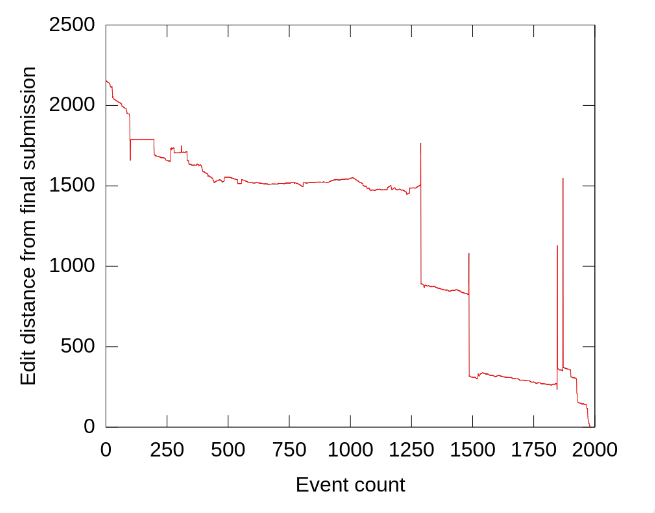
\includegraphics[scale=.25]{img/ed-a}
    \caption{Kasus A}\label{fig:edit-distance-a}
  \end{subfigure}%
  \begin{subfigure}{.5\linewidth}
    \centering
    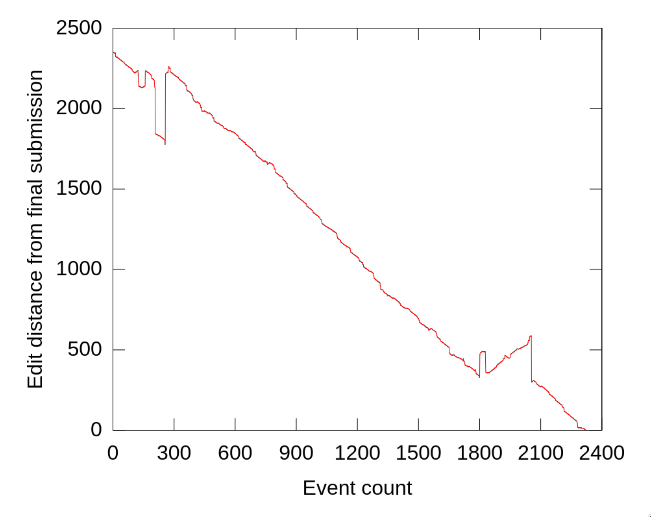
\includegraphics[scale=.25]{img/ed-b}
    \caption{Kasus B}\label{fig:edit-distance-b}
  \end{subfigure}\\[1ex]
  \begin{subfigure}{\linewidth}
    \centering
    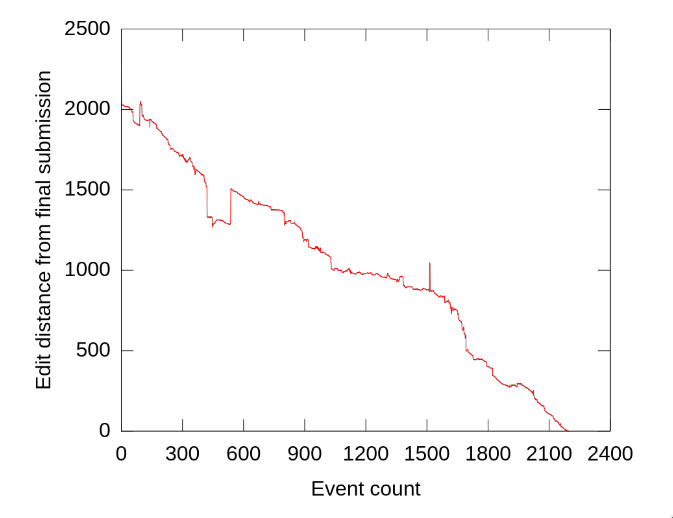
\includegraphics[scale=.25]{img/ed-c}
    \caption{Kasus C}\label{fig:edit-distance-c}
  \end{subfigure}
  \caption{Grafik \emph{edit-distance}}\label{fig:test}
\end{figure}

\section{Teknologi Pengembangan Perangkat Lunak}

\subsection{\emph{Python}}

\emph{Python} adalah bahasa pemrograman dengan \emph{syntax} yang elegan dan
sederhana yang dikembangkan oleh Guido van Rossum pada tahun 1990. \emph{Python}
bersifat \emph{interpreted} dan mendukung paradigma
\emph{object-oriented}. \emph{Python} juga memiliki dukungan struktur data
tingkat tinggi seperti \emph{dictionaries} dan \emph{list}. Berbeda dengan
bahasa \emph{scripting} yang lain, \emph{Python} dapat digunakan secara gratis,
bahkan untuk tujuan komersial \parencite{sanner1999python}.

\subsection{\emph{Git (Distributed Version Control)}}

\emph{Distributed version control} merupakan sebuah konsep di mana
aplikasi \emph{version control} dapat merekam semua perubahan yang
terjadi pada sebuah berkas secara terdistribusi atau tidak terpusat.
Sifatnya yang tidak terpusat memiliki kelebihan untuk melakukan semua
operasi secara lokal. Berbeda dengan \emph{version control} lainnya yang menggunakan \emph{diff}
untuk menyimpan berkas dari suatu waktu ke waktu, \emph{git} menggunakan
model \emph{snapshot} atau merekam seluruh berkas pada suatu waktu
tertentu. Hal ini memiliki kelebihan seperti kecepatan dalam
konstruksi berkas yang diminta pada waktu tertentu. Pada mulanya
\emph{git} dikembangkan oleh Linus Torvalds pada tahun 2005, Linus
kemudian menunjuk Junio Hamano untuk menjadi \emph{maintainer} hingga
sekarang \parencite{chacon2014pro}. \emph{Git} sejak awal diciptakan
secara modern sehingga memiliki integritas menggunakan \emph{hash}
\emph{SHA1} yang berupa 40 karakter heksadesimal. Hal ini yang
dijelaskan oleh Linus Torvalds sebagai \emph{content adressable}
layaknya \emph{filesystem} \parencite{gitmail1}. Tabel Kode~\ref{code:git-saved}
menunjukkan perintah pada \emph{git} untuk menyimpan perubahan suatu
berkas.

\par\null\par
\begin{code}
\begin{ignasicblock}[title=commit,minted language=text]
git commit -m "saved"
\end{ignasicblock}
  \captionof{listing}{Perintah untuk menyimpan perubahan pada
    \emph{git}}\label{code:git-saved}
\end{code}

\subsection{\emph{Qt (Widget Toolkit)}}

\emph{Qt} merupakan pustaka yang digunakan untuk membangun
\emph{graphical user interface}. Awalnya \emph{Qt} dikembangan oleh
Haavard Nord dan Eirik Chambe-Eng. Pada saat ini \emph{Qt}
dikembangan oleh \emph{The Qt Company} \parencite{qthistory}.
\emph{Qt} memiliki beberapa lisensi, di antaranya lisensi komersial dan
lisensi \emph{GPL 2.0}. Modul-modul yang dimiliki \emph{Qt} di antaranya adalah
\emph{Qt Core, Qt GUI,} dan \emph{Qt Widgets}
\parencite{qtabout}. Secara umum \emph{Qt} digunakan untuk
membangun \emph{graphical user interface} agar memudahkan interaksi
pengguna dengan aplikasi. Terlihat pada gambar~\ref{fig:hello-window} \emph{Qt} digunakan
untuk membuat \emph{window} sederhana dengan menggunakan kode pada
Tabel Kode~\ref{code:hello-window}.

\par\null\par
\begin{code}
\begin{ignasicblock}[title=hello,minted language=python]
import sys
from PyQt5.QtWidgets import QApplication, QWidget

if __name__ == '__main__':
    app = QApplication(sys.argv)
    window = QWidget()
    window.resize(250, 150)
    window.setWindowTitle('Hello World')
    window.show()
    sys.exit(app.exec_())
\end{ignasicblock}
  \captionof{listing}{Kode untuk membuat \emph{window} sederhana}\label{code:hello-window}
\end{code}

\begin{figure}[tph]
  \centering
  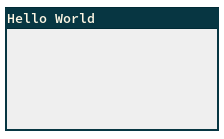
\includegraphics[width=.4\linewidth]{img/hello-window}
  \caption{\emph{Window} sederhana dengan \emph{Qt}}\label{fig:hello-window}
\end{figure}

\subsection{\emph{Draw.io}}

\emph{Draw.io} merupakan sebuah kakas bantu untuk menggambar
diagram ataupun \emph{mock up}. \emph{Draw.io} memiliki lisensi perangkat lunak bebas (\emph{Apache
  v2}) dan dapat diakses melalui peramban secara daring. \emph{Draw.io} dibangun
oleh Gaudenz Alder menggunakan bahasa pemrograman \emph{javascript} pada tahun 2000. Peramban
yang didukung diantaranya \emph{IE 11, Chrome 32+, Firefox 38+, Safari 9.1.x,}
dan \emph{Opera 20+} \parencite{drawio}.

%%% Local Variables:
%%% coding: utf-8
%%% mode: latex
%%% TeX-engine: xetex
%%% TeX-master: "skripsi"
%%% ispell-local-dictionary: "id"
%%% End:
